%%%%%%%%%%%%%%%%%%%%%%%%%%%%%%%%%%%%%%%%%%%%%%%%%%%%%%%%%%%%%%%%%%%%%%%%%%%%%%%%%%
\begin{frame}[fragile]\frametitle{Abstract}

Graph query languages, while precise and powerful, can sometimes be challenging to comprehend and employ. 
However, employing natural language to construct and query graphs presents an ideal alternative. 
This approach is particularly suitable for Knowledge Graphs derived from textual data. 
This presentation explores the foundation, methodologies, and illustrative instances of utilizing LLMs to enhance KGs.


\end{frame}

%%%%%%%%%%%%%%%%%%%%%%%%%%%%%%%%%%%%%%%%%%%%%%%%%%%%%%%%%%%%%%%%%%%%%%%%%%%%%%%%%%
\begin{frame}[fragile]\frametitle{}
\begin{center}
{\Large Knowledge Graph (KG)}

\end{center}
\end{frame}

%%%%%%%%%%%%%%%%%%%%%%%%%%%%%%%%%%%%%%%%%%%%%%%%%%%%%%%%%%%%%%%%%%%%%%%%%%%%%%%%%%
%%%%%%%%%%%%%%%%%%%%%%%%%%%%%%%%%%%%%%%%%%%%%%%%%%%%%%%%%%%
\begin{frame}[fragile]\frametitle{What is KG?}

\begin{itemize}
\item A knowledge graph is a graph-based database that represents knowledge in a structured and semantically rich format. 
\item This could be generated by extracting entities and relationships from structured or unstructured data, such as text from documents. 
\item A key requirement for maintaining data quality in a knowledge graph is to base it on standard ontology. 
\item Having a standardized ontology often involves the cost of incorporating this ontology in the software development cycle.
\end{itemize}

\end{frame}

%%%%%%%%%%%%%%%%%%%%%%%%%%%%%%%%%%%%%%%%%%%%%%%%%%%%%%%%%%%
\begin{frame}[fragile]\frametitle{Populating KG}

\begin{center}
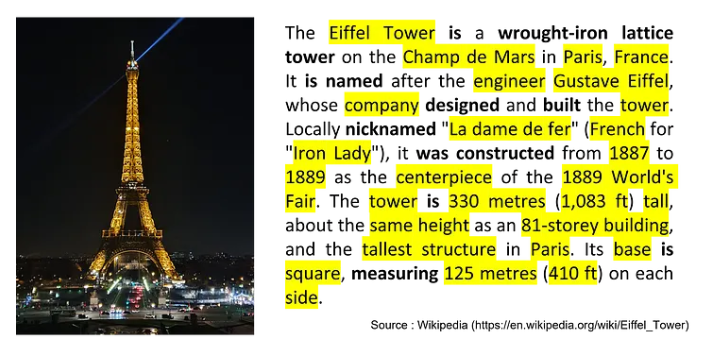
\includegraphics[width=\linewidth,keepaspectratio]{llm48}
\end{center}

{\tiny (Ref: Automatic Knowledge Graphs: The Impossible Grail - Patrick Meyer)}

\end{frame}

%%%%%%%%%%%%%%%%%%%%%%%%%%%%%%%%%%%%%%%%%%%%%%%%%%%%%%%%%%%
\begin{frame}[fragile]\frametitle{Populating KG}

\begin{itemize}
\item The Eiffel Tower is a wrought-iron lattice tower.
\item The Eiffel Tower is located on the Champ de Mars.
\item The Champ de Mars is located in Paris.
\item Paris is located in France.
\item The Eiffel Tower is named after the engineer Gustave Eiffel.
\item Gustave Eiffel’s company designed the Eiffel Tower.
\item Gustave Eiffel’s company built the Eiffel Tower.
\item The Eiffel Tower is locally nicknamed “La dame de fer”.
\item “La dame de fer” is the French for ”The Iron Lady”
\item The Eiffel Tower was constructed from 1887 to 1889.
\item The Eiffel Tower was constructed as the centerpiece of the 1889 World’s Fair.
\item The Eiffel Tower is 330 meters high.
\item The Eiffel Tower is the same height as an 81-storey building.
\item The Eiffel Tower is the tallest structure in Paris.
\item The base of the Eiffel Tower is a square.
\item The base of the Eiffel Tower measures 125 meters on each side.epresenting conceptual understanding, establishing connections between the LLM's numerical vectors and the KG's ontological classes.
\end{itemize}

{\tiny (Ref: Automatic Knowledge Graphs: The Impossible Grail - Patrick Meyer)}

\end{frame}

%%%%%%%%%%%%%%%%%%%%%%%%%%%%%%%%%%%%%%%%%%%%%%%%%%%%%%%%%%%
\begin{frame}[fragile]\frametitle{Populating KG}

\begin{center}
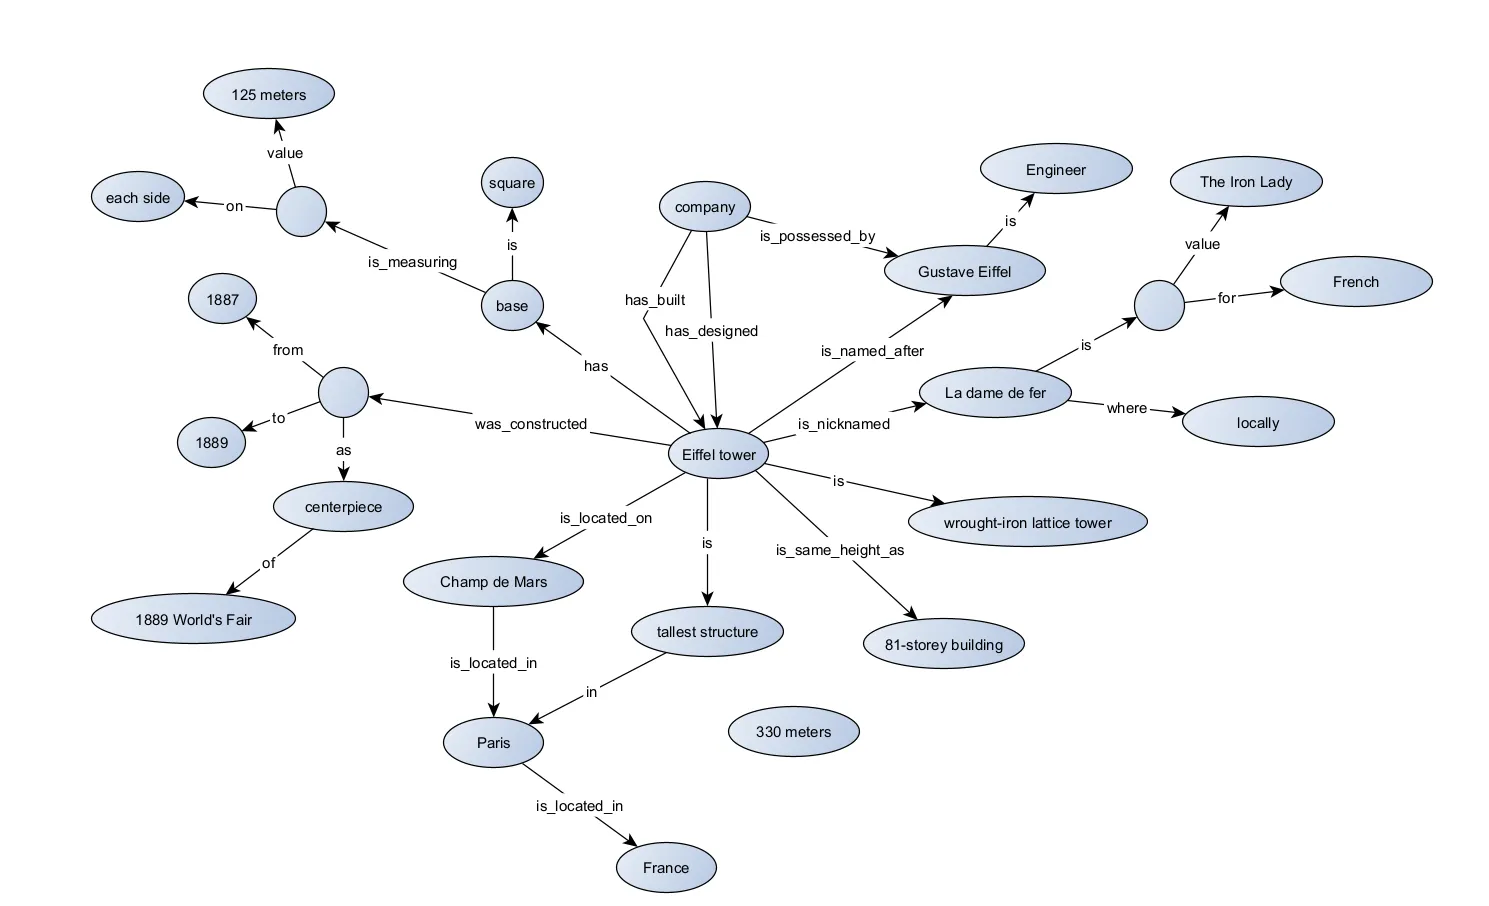
\includegraphics[width=\linewidth,keepaspectratio]{llm49}
\end{center}

{\tiny (Ref: Automatic Knowledge Graphs: The Impossible Grail - Patrick Meyer)}

\end{frame}

%%%%%%%%%%%%%%%%%%%%%%%%%%%%%%%%%%%%%%%%%%%%%%%%%%%%%%%%%%%
\begin{frame}[fragile]\frametitle{Populating KG is not easy}

\begin{center}
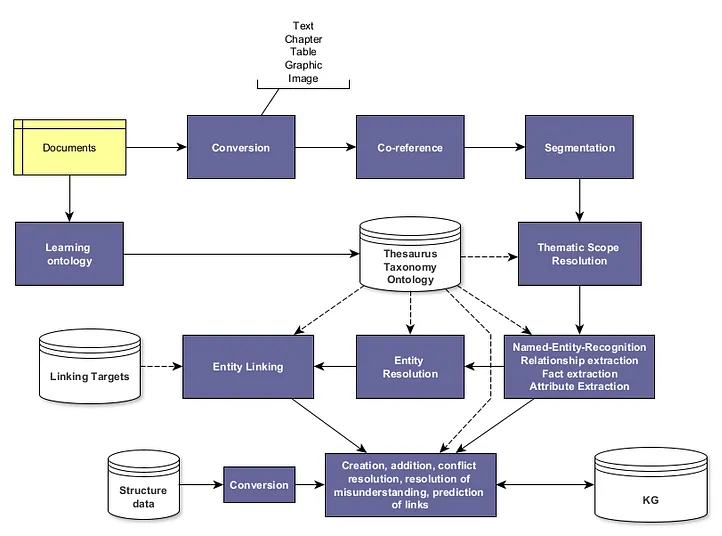
\includegraphics[width=\linewidth,keepaspectratio]{llm50}
\end{center}

{\tiny (Ref: Automatic Knowledge Graphs: The Impossible Grail - Patrick Meyer)}

\end{frame}

%%%%%%%%%%%%%%%%%%%%%%%%%%%%%%%%%%%%%%%%%%%%%%%%%%%%%%%%%%%%%%%%%%%%%%%%%%%%%%%%%%
%%%%%%%%%%%%%%%%%%%%%%%%%%%%%%%%%%%%%%%%%%%%%%%%%%%%%%%%%%%
\begin{frame}[fragile]\frametitle{What is LLM?}

\begin{itemize}
\item Large Language Models (LLMs): Machine learning algorithms for interpreting, translating, and summarizing natural language texts.
\item Size: Span hundreds of gigabytes with trillions of parameters.
\item Deep neural networks: Learn from extensive training data to generate appropriate outputs.
\item Self-attention mechanisms: Capture relationships between words, even with incorrect positioning.
\item Transformer architecture: Implements self-attention mechanisms.
\item Training data: Accumulated from multiple sources (books, internet, articles, social media, research papers).
\item Applications: Conversational AI, content creation engines, search engines, customer service agents, etc.
Enhance natural language processing tasks.
\end{itemize}

\end{frame}


%%%%%%%%%%%%%%%%%%%%%%%%%%%%%%%%%%%%%%%%%%%%%%%%%%%%%%%%%%%%%%%%%%%%%%%%%%%%%%%%%%
\begin{frame}[fragile]\frametitle{}
\begin{center}
{\Large Knowledge Graph + Language Model}

\end{center}
\end{frame}


%%%%%%%%%%%%%%%%%%%%%%%%%%%%%%%%%%%%%%%%%%%%%%%%%%%%%%%%%%%%%%%%%%%%%%%%%%%%%%%%%%
%%%%%%%%%%%%%%%%%%%%%%%%%%%%%%%%%%%%%%%%%%%%%%%%%%%%%%%%%%%
\begin{frame}[fragile]\frametitle{How Can Knowledge Graphs and LLMs Work Together?}

\begin{itemize}
\item Knowledge graphs + Large Language Models (LLMs): Powerful solution to overcome LLM limitations.
\item Address hallucination problem: Improves query result accuracy.
\item Integrating knowledge graph with LLM: Incorporates contextual knowledge base.
\item Enables logical connections between concepts.
\item Utilizes structured and unstructured data.
\item Generates more accurate and relevant outputs.
\item Enhances reasoning and understanding.
\item Produces more meaningful text.
\end{itemize}

\end{frame}

%%%%%%%%%%%%%%%%%%%%%%%%%%%%%%%%%%%%%%%%%%%%%%%%%%%%%%%%%%%%%%%%%%%%%%%%%%%%%%%%%%
%%%%%%%%%%%%%%%%%%%%%%%%%%%%%%%%%%%%%%%%%%%%%%%%%%%%%%%%%%%
\begin{frame}[fragile]\frametitle{Why?}

\begin{itemize}
\item KnowledgeGraphs: Excellent for representing domain data.
\item Deliver answers through expert-formulated queries.
\item Large Language Models (LLMs): Allow any user to ask questions.
\item Retrieve comprehensive answers.
\item LLM answers lack user-specific information.
\end{itemize}
	
So, combining both will be a Win-Win situation.

{\tiny (Ref: Knowledge Graphs + Large Language Models = The ability for users to ask their own questions? - Peter Lawrence)}

\end{frame}

%%%%%%%%%%%%%%%%%%%%%%%%%%%%%%%%%%%%%%%%%%%%%%%%%%%%%%%%%%%
\begin{frame}[fragile]\frametitle{What?}

Solution: 

\begin{itemize}
\item LLM converts verbose query to GraphQL syntax.
\item GraphQL performs information retrieval.
\item LLM converts GraphQL response to verbose answer.
\end{itemize}

	
{\tiny (Ref: Knowledge Graphs + Large Language Models = The ability for users to ask their own questions? - Peter Lawrence)}

\end{frame}

%%%%%%%%%%%%%%%%%%%%%%%%%%%%%%%%%%%%%%%%%%%%%%%%%%%%%%%%%%%
\begin{frame}[fragile]\frametitle{How?}

\begin{itemize}
\item Query : \lstinline|How is Valve-104 connected to Reflux-401?|
\item Using the OpenAI gpt-3.5-turbo LLM, provide the ontology of the RDF graph as the context prompt for the LLM.
\item Ask it to prepare some SPARQL
\end{itemize}	

\begin{lstlisting}
Sure! Here is an example of a SPARQL query that returns the sequence of nodes that connect two particular nodes, assuming that there is a unique path between them:
```
PREFIX connectivity: <http://example.org/ontology#>
SELECT ?path
WHERE {
  {
    <http://example.org/node1> (connectivity:connectedTo)+ ?path .
    ?path connectivity:connectedTo <http://example.org/node2> .
  }
}
```
\end{lstlisting}

\end{frame}

%%%%%%%%%%%%%%%%%%%%%%%%%%%%%%%%%%%%%%%%%%%%%%%%%%%%%%%%%%%
\begin{frame}[fragile]\frametitle{How?}

\begin{itemize}
\item Property path syntax: Find paths connecting two nodes.
\item \lstinline|(connectivity:connectedTo)+|: Traverses arbitrary length path with "connectedTo" property.
\item Query result: \lstinline|"?path"| variable represents sequence of connecting nodes (as URIs).
\item Assumes unique path between nodes.
\item Multiple paths or cycles may result in multiple/incorrect results.
\end{itemize}	

\end{frame}

%%%%%%%%%%%%%%%%%%%%%%%%%%%%%%%%%%%%%%%%%%%%%%%%%%%%%%%%%%%
\begin{frame}[fragile]\frametitle{LLM + KG for Recommendations}

Augmenting company information from KG and adding it into the prompt for better results.

\begin{center}
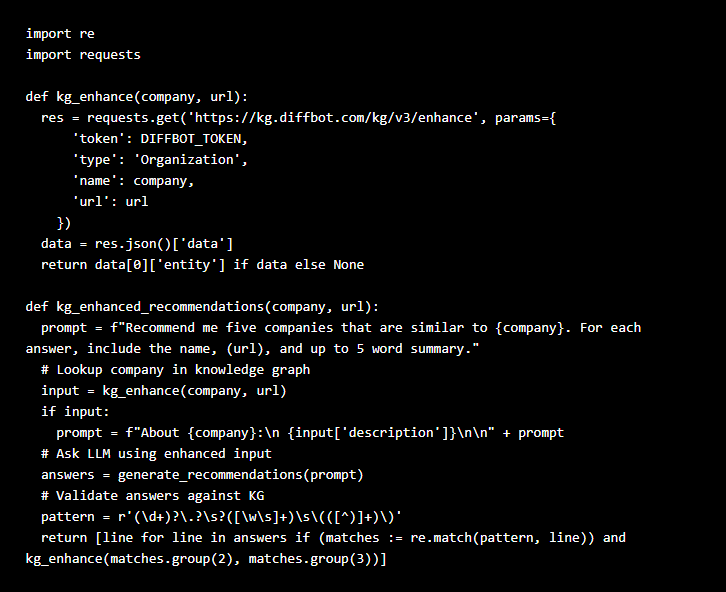
\includegraphics[width=0.5\linewidth,keepaspectratio]{llm51}
\end{center}	

{\tiny (Ref: Generating Company Recommendations using Large Language Models and Knowledge Graphs - Mike Tung)}

\end{frame}

%%%%%%%%%%%%%%%%%%%%%%%%%%%%%%%%%%%%%%%%%%%%%%%%%%%%%%%%%%%%%%%%%%%%%%%%%%%%%%%%%%
\begin{frame}[fragile]\frametitle{}
\begin{center}
{\Large Leveraging KG for Better LLM}
\end{center}
\end{frame}

%%%%%%%%%%%%%%%%%%%%%%%%%%%%%%%%%%%%%%%%%%%%%%%%%%%%%%%%%%%
\begin{frame}[fragile]\frametitle{How?}

\begin{itemize}
\item Large Language Models (LLMs), such as ChatGPT, have demonstrated immense potential in various applications but are limited by hallucinations, misinformation, and biases in enterprise contexts.
\item How integrating a graph-based Knowledge Graph as a support mechanism and interface can significantly improve the capabilities of LLMs?
\end{itemize}	

\end{frame}

%%%%%%%%%%%%%%%%%%%%%%%%%%%%%%%%%%%%%%%%%%%%%%%%%%%%%%%%%%%
\begin{frame}[fragile]\frametitle{Limitations of Large Language Models in the Enterprise Context}

\begin{itemize}
\item Hallucinations: LLMs generate plausible but inaccurate responses.
\item Misinformation: LLMs unintentionally perpetuate false information.
\item Biases: LLMs exhibit biases from training data, impacting decision-making.
\item Cut-off: LLMs lack awareness of events after their training.
\item Corpus: LLMs lack knowledge of events not in their training data.
\item Fine-tuning mitigates but doesn't eliminate hallucinations.
\item LLMs don't cite sources, lack access restrictions.
\end{itemize}	

\end{frame}

%%%%%%%%%%%%%%%%%%%%%%%%%%%%%%%%%%%%%%%%%%%%%%%%%%%%%%%%%%%
\begin{frame}[fragile]\frametitle{Solution for Limitations}

\begin{itemize}
\item Fine-tuning: Supervised training phase to optimize LLM performance.
\item Use case 1: Updating and expanding internal knowledge.
\item Use case 2: Fine-tuning for specific tasks (e.g., summarization, translation).
\end{itemize}	

\end{frame}


%%%%%%%%%%%%%%%%%%%%%%%%%%%%%%%%%%%%%%%%%%%%%%%%%%%%%%%%%%%
\begin{frame}[fragile]\frametitle{Graph-based Knowledge Graphs as Support Mechanisms for LLMs}

\begin{itemize}
\item Knowledge Graphs: Structured representation using nodes and edges.
\item Interface with LLMs: Integrates Knowledge Graphs with LLMs.
\item Enables access to structured data.
\item Enhances LLM outputs.
\item Benefits of Integration: Mitigates LLM limitations.
\item Provides accurate, context-specific, unbiased information.
\end{itemize}	

\end{frame}


%%%%%%%%%%%%%%%%%%%%%%%%%%%%%%%%%%%%%%%%%%%%%%%%%%%%%%%%%%%
\begin{frame}[fragile]\frametitle{KG as LLM Pre-training Corpora}

\begin{itemize}
\item KGs: Factual nature, extracted from trusted sources.
\item Post-processing and human editors ensure accuracy.
\item Advantages of incorporating KGs: Improved factual accuracy, reduced toxicity.
\item Integration challenge: Different structural format from pre-training corpora in language models.
\end{itemize}	

{\tiny (Ref: KELM: Integrating Knowledge Graphs with Language Model Pre-training Corpora - Siamak Shakeri, Oshin Agarwal)}
\end{frame}


%%%%%%%%%%%%%%%%%%%%%%%%%%%%%%%%%%%%%%%%%%%%%%%%%%%%%%%%%%%
\begin{frame}[fragile]\frametitle{Steps}

\begin{itemize}
\item  KGs: Factual info in structured [subject, relation, object] triples.
\item  Entity subgraph: Group of related triples.
\item  Data-to-text generation: Converts subgraphs to natural language text.
\item  NLP task for KG-based text generation.
\end{itemize}

\begin{center}
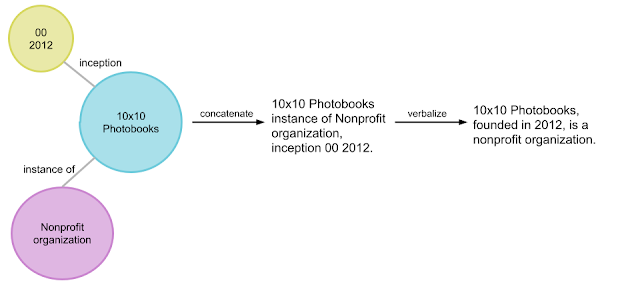
\includegraphics[width=0.5\linewidth,keepaspectratio]{llm47}
\end{center}	

{\tiny (Ref: KELM: Integrating Knowledge Graphs with Language Model Pre-training Corpora - Siamak Shakeri, Oshin Agarwal)}
\end{frame}




%%%%%%%%%%%%%%%%%%%%%%%%%%%%%%%%%%%%%%%%%%%%%%%%%%%%%%%%%%%%%%%%%%%%%%%%%%%%%%%%%%
\begin{frame}[fragile]\frametitle{}
\begin{center}
{\Large Leveraging LLM for Better KG}

\end{center}
\end{frame}

%%%%%%%%%%%%%%%%%%%%%%%%%%%%%%%%%%%%%%%%%%%%%%%%%%%%%%%%%%%%%%%%%%%%%%%%%%%%%%%%%%
%%%%%%%%%%%%%%%%%%%%%%%%%%%%%%%%%%%%%%%%%%%%%%%%%%%%%%%%%%%
\begin{frame}[fragile]\frametitle{How?}

\begin{itemize}
\item Knowledge graph generation: Systematic approach for organizations.
\item Step 1: Ingest standard ontology (e.g., insurance risk).
\item Use LLM (e.g., GPT-3) to script and populate graph database.
\item Step 2: LLM acts as intermediate layer for natural language queries.
\item Customized creation and search queries on the graph.
\item Platform customization (e.g., Neo4j).
\end{itemize}
\end{frame}

%%%%%%%%%%%%%%%%%%%%%%%%%%%%%%%%%%%%%%%%%%%%%%%%%%%%%%%%%%%
\begin{frame}[fragile]\frametitle{Steps}

\begin{center}
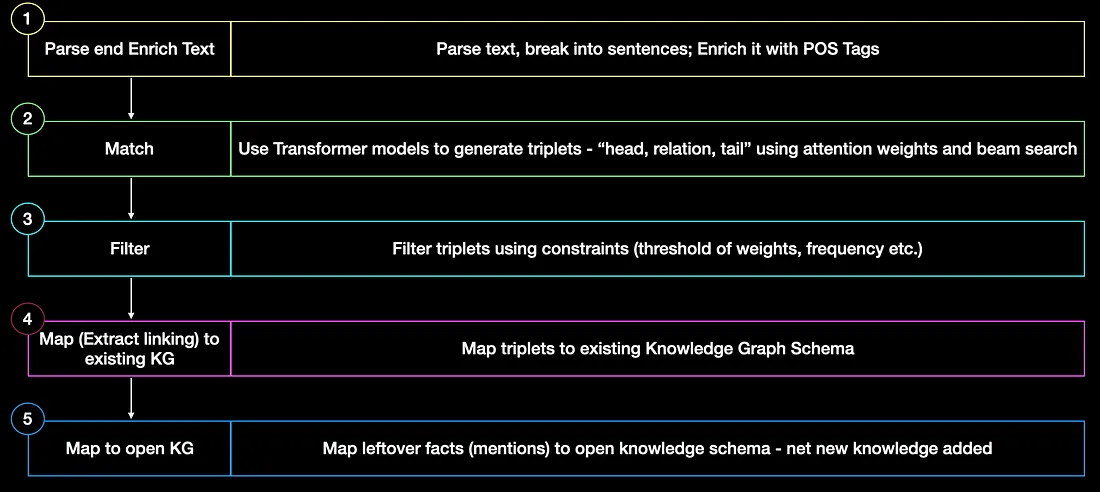
\includegraphics[width=0.5\linewidth,keepaspectratio]{llm52}
\end{center}	

{\tiny (Ref: Language Models are Open Knowledge Graphs .. but are hard to mine! - Nikhil Dharap)}
\end{frame}



%%%%%%%%%%%%%%%%%%%%%%%%%%%%%%%%%%%%%%%%%%%%%%%%%%%%%%%%%%%%%%%%%%%%%%%%%%%%%%%%%%
%%%%%%%%%%%%%%%%%%%%%%%%%%%%%%%%%%%%%%%%%%%%%%%%%%%%%%%%%%%
\begin{frame}[fragile]\frametitle{Steps}

\begin{itemize}
\item Study ontology, identify entities and relations.
\item Build text prompt for LLM to generate schema and database.
\item Prompt includes ontology description, entities, relationships.
\item Clearly described in natural language for LLM understanding.
\item Include constraints (data types, unique/foreign keys).
\item Text prompt used as input for LLM to generate Cypher query.\end{itemize}
\end{frame}



%%%%%%%%%%%%%%%%%%%%%%%%%%%%%%%%%%%%%%%%%%%%%%%%%%%%%%%%%%%
\begin{frame}[fragile]\frametitle{Work-flow}

\begin{center}
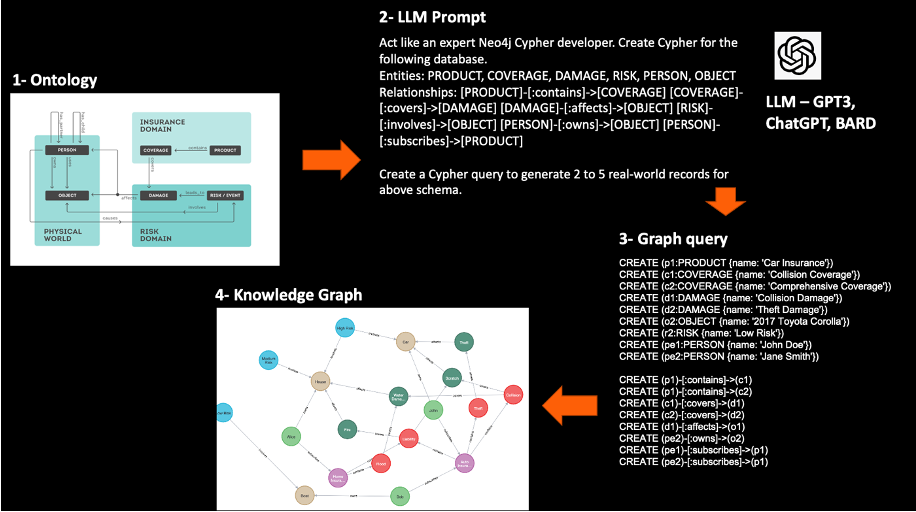
\includegraphics[width=\linewidth,keepaspectratio]{llm46}

{\tiny (Ref: How to use large language models and knowledge graphs to manage enterprise data - Dattaraj Rao, Persistent Systems)}
\end{center}
\end{frame}


%%%%%%%%%%%%%%%%%%%%%%%%%%%%%%%%%%%%%%%%%%%%%%%%%%%%%%%%%%%%%%%%%%%%%%%%%%%%%%%%%%
%%%%%%%%%%%%%%%%%%%%%%%%%%%%%%%%%%%%%%%%%%%%%%%%%%%%%%%%%%%
\begin{frame}[fragile]\frametitle{Pros and Cons}

\begin{itemize}
\item Standardization: Ensures consistent and standardized data.
\item Efficiency: Saves time and resources, ensures correct queries.
\item Intuitive querying: Reduces need for deep graph understanding.
\item Productivity: Updates knowledge graph with new data.
\item Modified Cypher query adds new nodes and edges.
\item Updated query ingested into graph database.
\end{itemize}
\end{frame}


%%%%%%%%%%%%%%%%%%%%%%%%%%%%%%%%%%%%%%%%%%%%%%%%%%%%%%%%%%%%%%%%%%%%%%%%%%%%%%%%%%
\begin{frame}[fragile]\frametitle{}
\begin{center}
{\Large Characteristics of KG + LLMs}

{\tiny (Ref: LinkedIn posts by Tony Seale)}
\end{center}
\end{frame}

%%%%%%%%%%%%%%%%%%%%%%%%%%%%%%%%%%%%%%%%%%%%%%%%%%%%%%%%%%%
\begin{frame}[fragile]\frametitle{Training data for GPT}

\begin{itemize}
\item GPT learns from web pages, with 40\% containing JSON-LD islands.
\item Reverse relationship: Use islands to connect GPT's embeddings to internal data.
\end{itemize}
	  
\end{frame}

%%%%%%%%%%%%%%%%%%%%%%%%%%%%%%%%%%%%%%%%%%%%%%%%%%%%%%%%%%%
\begin{frame}[fragile]\frametitle{Transformers as GNNs}

\begin{itemize}
\item Transformers: Analyze sentences by assigning word importance.
\item Attention mechanism: Evaluates pairwise interactions between tokens.
\item Interactions represented as edges in a complete graph.
\item Transformers as graph-based models: Tokens as nodes, attention weights as edges.
\end{itemize}
	  
\end{frame}


%%%%%%%%%%%%%%%%%%%%%%%%%%%%%%%%%%%%%%%%%%%%%%%%%%%%%%%%%%%
\begin{frame}[fragile]\frametitle{Transparency and Explainability}

\begin{itemize}
\item Language models (e.g., ChatGPT) provide answers in interconnected node graphs.
\item Visualizing connections reveals decision-making process.
\item Helps address biases and ensure regulatory compliance.
\end{itemize}
	  
\end{frame}

%%%%%%%%%%%%%%%%%%%%%%%%%%%%%%%%%%%%%%%%%%%%%%%%%%%%%%%%%%%
\begin{frame}[fragile]\frametitle{Knowledge Management and Control}

\begin{itemize}
\item Language models (e.g., ChatGPT) provide answers in interconnected node graphs.
\item Visualizing connections reveals decision-making process.
\item Helps address biases and ensure regulatory compliance.
\end{itemize}
	  
\end{frame}

%%%%%%%%%%%%%%%%%%%%%%%%%%%%%%%%%%%%%%%%%%%%%%%%%%%%%%%%%%%
\begin{frame}[fragile]\frametitle{Alignment with Ontological Worldview}

\begin{itemize}
\item Leverage Knowledge Graph ontology to constrain the language model.
\item Alignment maintains logical consistency with organization's perspective.
\item Prevents retrieval of outdated or incorrect information.
\end{itemize}
	  
\end{frame}

%%%%%%%%%%%%%%%%%%%%%%%%%%%%%%%%%%%%%%%%%%%%%%%%%%%%%%%%%%%
\begin{frame}[fragile]\frametitle{Alignment with Ontological Worldview}
\begin{itemize}
\item Knowledge Graph ontology constrains language model.
\item Alignment ensures logical consistency with organization's perspective.
\item Prevents retrieval of outdated or incorrect information.
\end{itemize}
\end{frame}

%%%%%%%%%%%%%%%%%%%%%%%%%%%%%%%%%%%%%%%%%%%%%%%%%%%%%%%%%%%
\begin{frame}[fragile]\frametitle{Risk Assessment and Compliance}
\begin{itemize}
\item Knowledge graphs enable comprehensive risk assessment.
\item Empower proactive identification of sensitive information, compliance risks, and ethical challenges.
\item Mitigate potential issues before escalation.
\end{itemize}
\end{frame}

%%%%%%%%%%%%%%%%%%%%%%%%%%%%%%%%%%%%%%%%%%%%%%%%%%%%%%%%%%%
\begin{frame}[fragile]\frametitle{Ethical and Fair AI}
\begin{itemize}
\item Knowledge graphs encode ethical guidelines and fairness constraints into Ontology that upholds organization's standards.
\item Language model adheres to ethical principles and promotes fairness.
\end{itemize}
\end{frame}

%%%%%%%%%%%%%%%%%%%%%%%%%%%%%%%%%%%%%%%%%%%%%%%%%%%%%%%%%%%
\begin{frame}[fragile]\frametitle{Challenges}
\begin{itemize}
\item Balancing innovation and risk management in rapidly evolving landscape
\item Language models like ChatGPT offer productivity and customer experience benefits
\item Robust governance frameworks are essential to mitigate risks
\end{itemize}
\end{frame}

%%%%%%%%%%%%%%%%%%%%%%%%%%%%%%%%%%%%%%%%%%%%%%%%%%%%%%%%%%%
\begin{frame}[fragile]\frametitle{Knowledge Graphs: A Safe Path Forward}
\begin{itemize}
\item Knowledge graphs: Safe and effective approach for harnessing language models
\item Leverage capabilities for navigating risk and governance
\item Unlock benefits of AI-driven language models
\end{itemize}
\end{frame}

%%%%%%%%%%%%%%%%%%%%%%%%%%%%%%%%%%%%%%%%%%%%%%%%%%%%%%%%%%%
\begin{frame}[fragile]\frametitle{Generalized or Specific}
\begin{itemize}
\item Large Language Models (LLMs): Generalization, flexibility, and creativity, but suffer from hallucinations, unreliability, and staleness.
\item Databases: Accuracy, speed, and reliability, but lack adaptability and intelligence.
\item Bridge the gap with graphs: Integrate LLMs with internal data through Knowledge Graphs.
\item Working Memory Graph (WMG): Combines strengths of LLMs and databases for tasks.
\item WMG construction: LLM processes question, returns node graph with URLs as identifiers.
\item Ground truths: Stored in the organization's Knowledge Graph, linked to URLs.
\item Conceptual understanding: WMG incorporates nodes connecting LLM's vectors and KG's classes.
\end{itemize}
\end{frame}


%%%%%%%%%%%%%%%%%%%%%%%%%%%%%%%%%%%%%%%%%%%%%%%%%%%%%%%%%%%
\begin{frame}[fragile]\frametitle{KG + LLM @ Neo4j}
\begin{itemize}
\item https://github.com/neo4j/NaLLM
\item Explore, develop, and showcase practical uses of LLMs with Neo4j data science algorithms.
\item Strategy can yield substantial breakthroughs for businesses.
\item Enhance accuracy, transparency, and predictability of model output.
\item Open up new use-cases for LLMs and databases.
\item Real-world use-cases:

	\begin{itemize}
	\item Natural Language Interface: "Talk to your database" with generated queries based on user questions and inferred database schema.
	\item Creating Knowledge Graph from Unstructured Data: LLMs decipher entities, discern relationships, and eliminate redundancies by recognizing duplicates.
	\end{itemize}

\end{itemize}
\end{frame}


%%%%%%%%%%%%%%%%%%%%%%%%%%%%%%%%%%%%%%%%%%%%%%%%%%%%%%%%%%%%%%%%%%%%%%%%%%%%%%%%%%
\begin{frame}[fragile]\frametitle{}
\begin{center}
{\Large Conclusions}

\end{center}
\end{frame}

%%%%%%%%%%%%%%%%%%%%%%%%%%%%%%%%%%%%%%%%%%%%%%%%%%%%%%%%%%%%%%%%%%%%%%%%%%%%%%%%%%
%%%%%%%%%%%%%%%%%%%%%%%%%%%%%%%%%%%%%%%%%%%%%%%%%%%%%%%%%%%
\begin{frame}[fragile]\frametitle{Benefits of Combining Knowledge Graphs and LLMs}

\begin{itemize}
\item LLMs:
	\begin{itemize}
	\item  Hallucinate.
	\item   Have general knowledge.
	\item   Understand natural language.
	\item   Do not provide structured responses.
	\end{itemize}

\item KGs:
	\begin{itemize}
	\item   Do not understand language.
	\item   Provide structured responses.
	\item   Are accurate and interpretable.
	\item   Have domain-specific knowledge.
	\end{itemize}

\item LLMs+KGs have the potential to overcome some of the weaknesses of LLMs.

\end{itemize}

{\tiny (Ref: LinkedIn post by Miguel Fierro)}


\end{frame}

%%%%%%%%%%%%%%%%%%%%%%%%%%%%%%%%%%%%%%%%%%%%%%%%%%%%%%%%%%%
\begin{frame}[fragile]\frametitle{Benefits of Combining Knowledge Graphs and LLMs}

\begin{center}
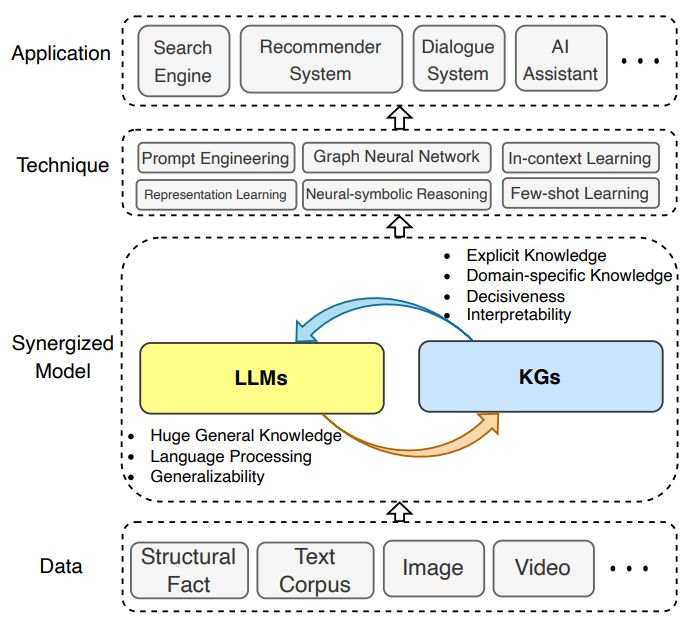
\includegraphics[width=\linewidth,keepaspectratio]{llm54}
\end{center}	

{\tiny (Ref: LinkedIn post by Miguel Fierro)}

	
\end{frame}

%%%%%%%%%%%%%%%%%%%%%%%%%%%%%%%%%%%%%%%%%%%%%%%%%%%%%%%%%%%
\begin{frame}[fragile]\frametitle{Awesome-LLM-KG Github repo}

\begin{center}
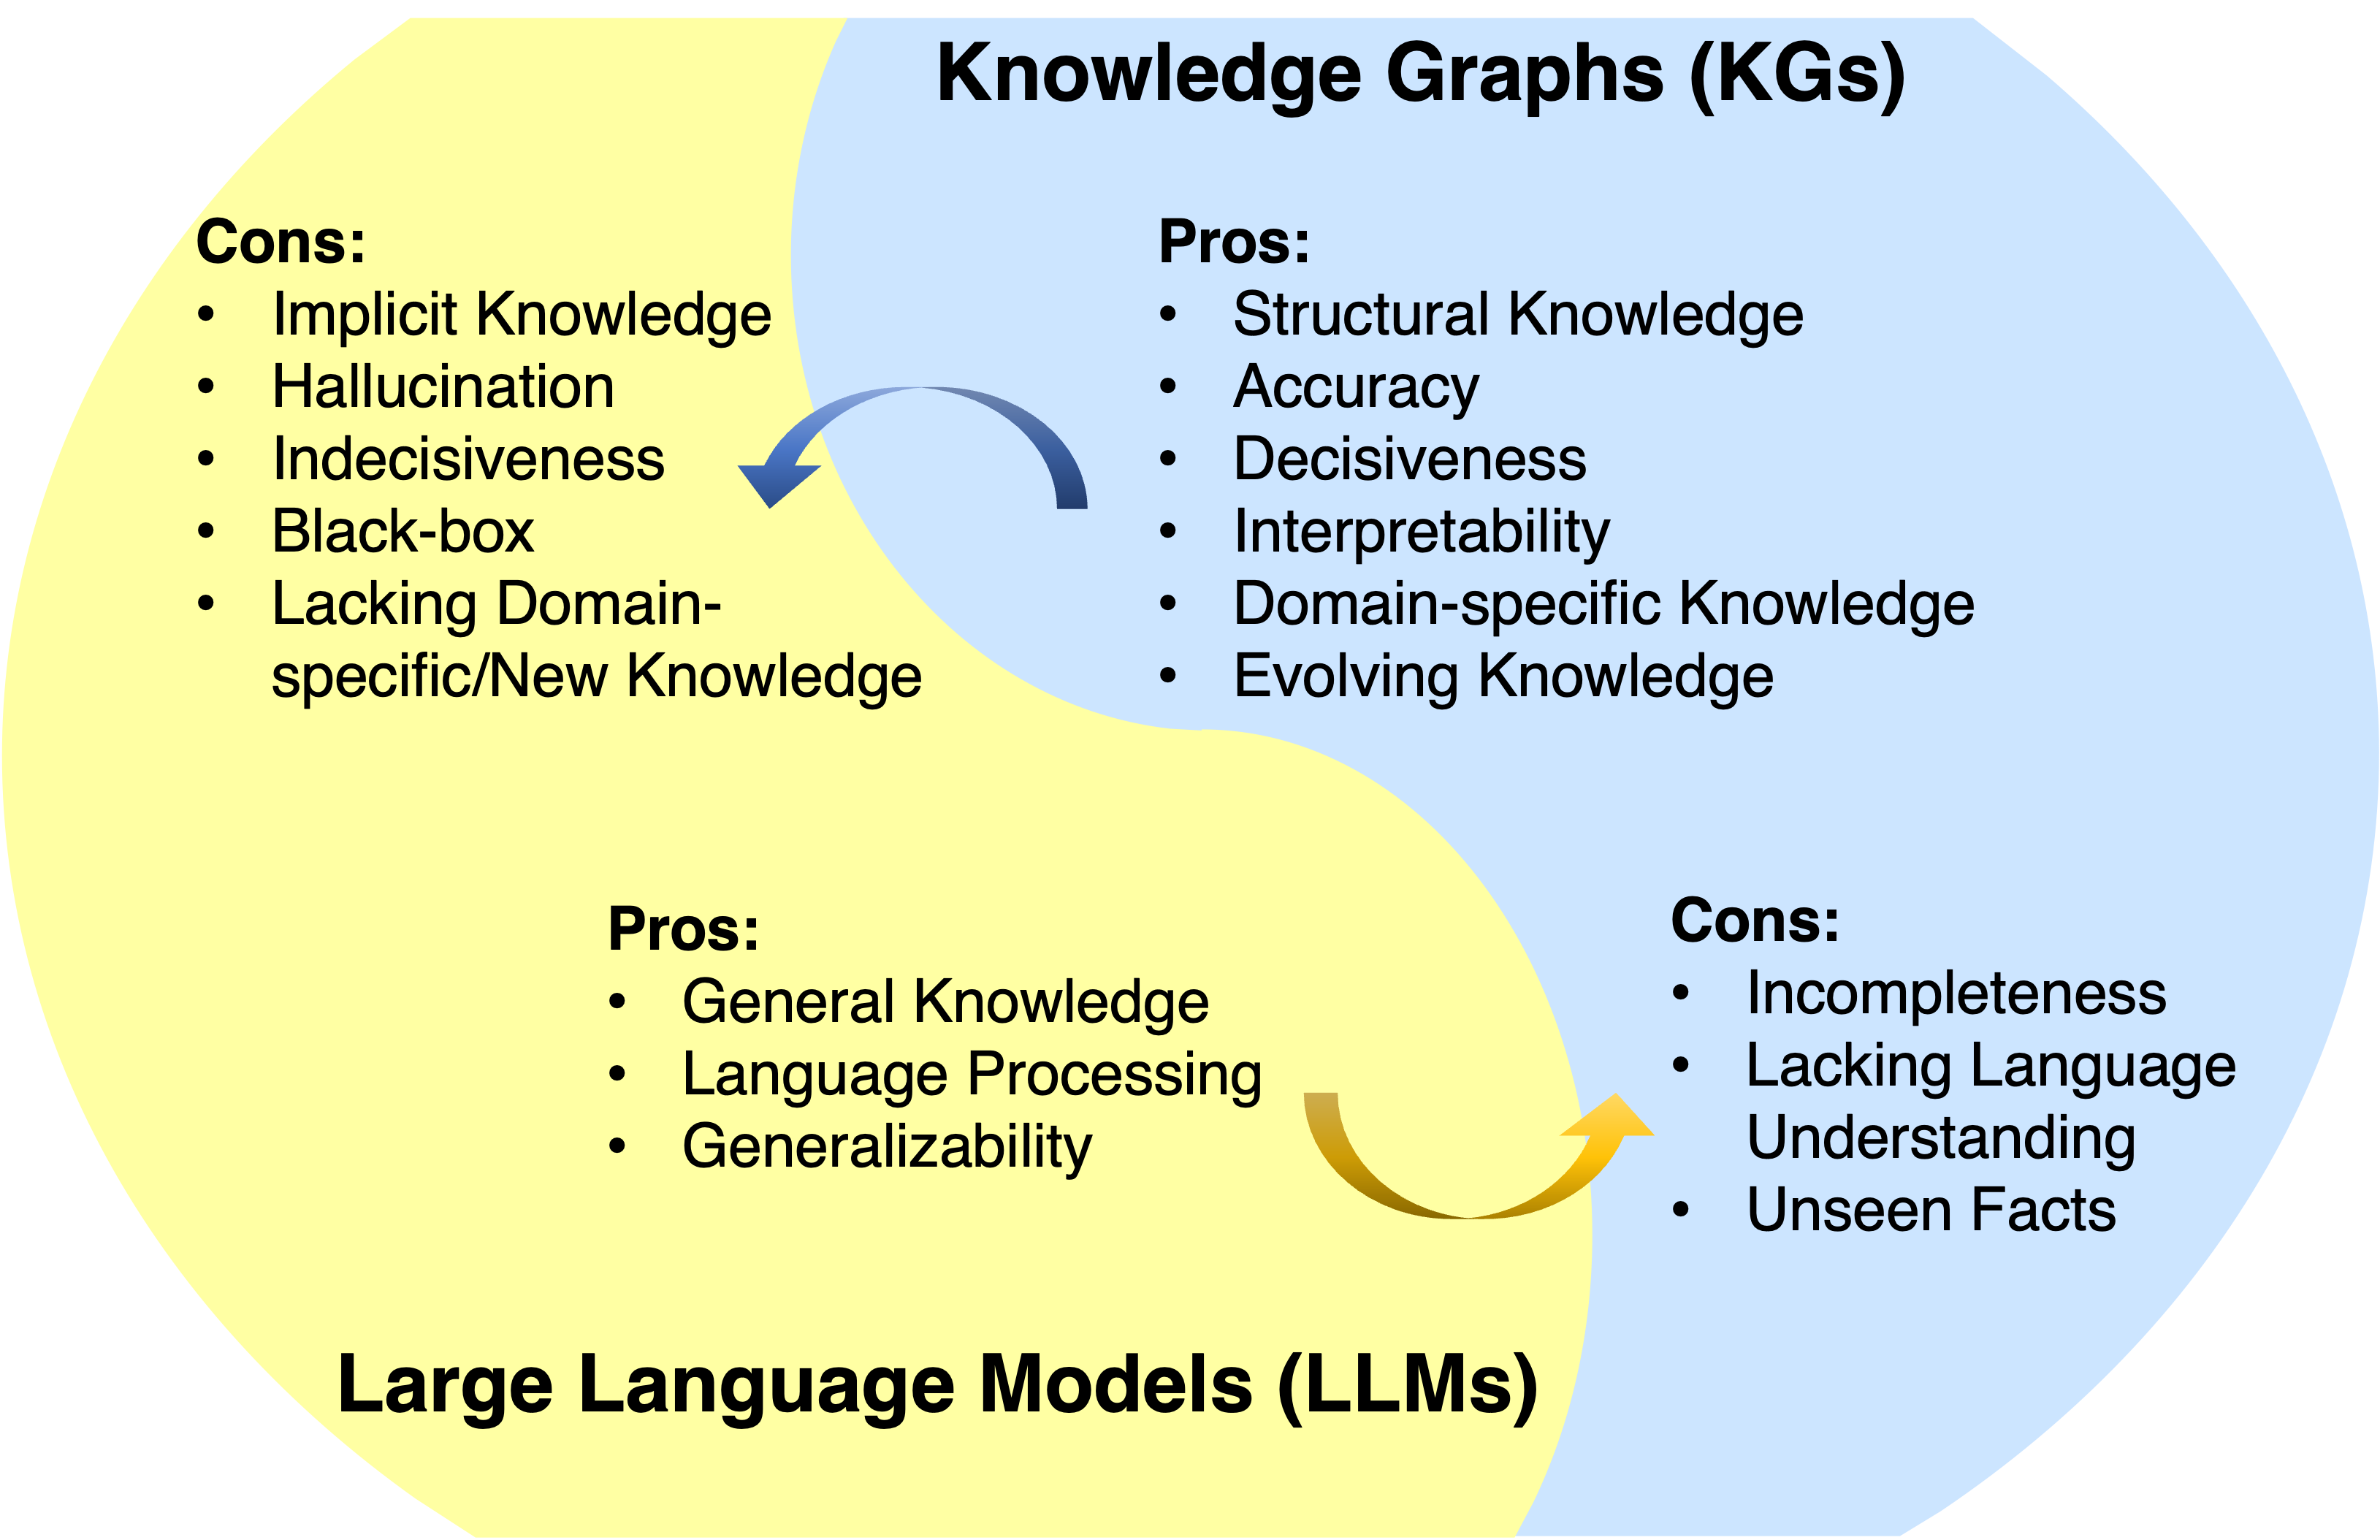
\includegraphics[width=\linewidth,keepaspectratio]{llm55}
\end{center}	

{\tiny (Ref: https://github.com/RManLuo/Awesome-LLM-KG)}

	
\end{frame}

%%%%%%%%%%%%%%%%%%%%%%%%%%%%%%%%%%%%%%%%%%%%%%%%%%%%%%%%%%%
\begin{frame}[fragile]\frametitle{Awesome-LLM-KG Github repo}

\begin{center}
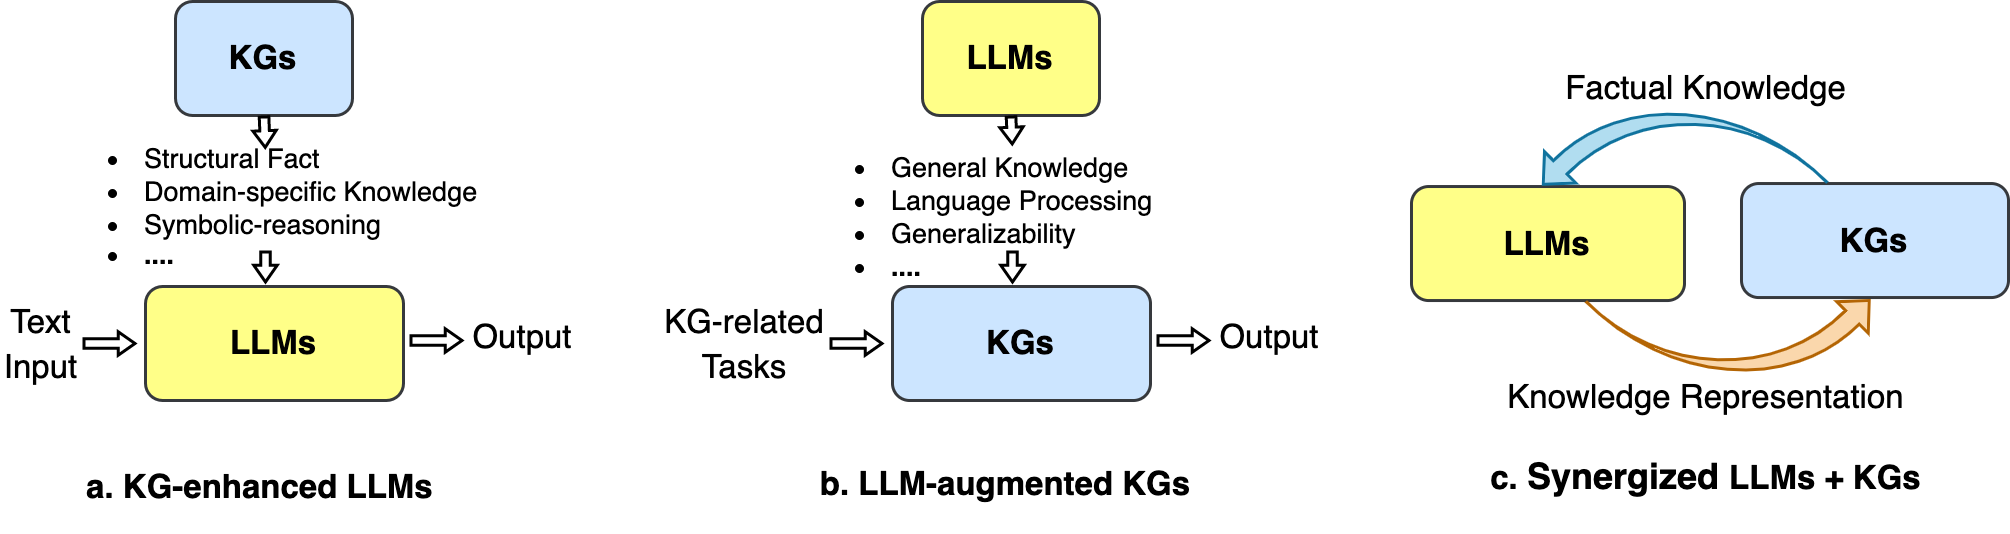
\includegraphics[width=\linewidth,keepaspectratio]{llm56}
\end{center}	

{\tiny (Ref: https://github.com/RManLuo/Awesome-LLM-KG)}

	
\end{frame}



%%%%%%%%%%%%%%%%%%%%%%%%%%%%%%%%%%%%%%%%%%%%%%%%%%%%%%%%%%%%%%%%%%%%%%%%%%%%%%%%%%
%%%%%%%%%%%%%%%%%%%%%%%%%%%%%%%%%%%%%%%%%%%%%%%%%%%%%%%%%%%
\begin{frame}[fragile]\frametitle{Benefits of Combining Knowledge Graphs and LLMs}

\begin{itemize}
\item Centralized source of accurate knowledge
\item Structured knowledge fusion of information in different formats
\item Increased informative value of collected data
\item Gives LLMs a human reference frame of the real-world
\end{itemize}

\end{frame}

%%%%%%%%%%%%%%%%%%%%%%%%%%%%%%%%%%%%%%%%%%%%%%%%%%%%%%%%%%%%%%%%%%%%%%%%%%%%%%%%%%
%%%%%%%%%%%%%%%%%%%%%%%%%%%%%%%%%%%%%%%%%%%%%%%%%%%%%%%%%%%
\begin{frame}[fragile]\frametitle{What's next \ldots}

\begin{itemize}
\item Chain of Thought:
	\begin{itemize}
	\item LLM determines necessary steps
	\item Executes them sequentially
	\end{itemize}
	
\item Tree of Thought:
	\begin{itemize}
	\item Combines thought with symbolic tree search algorithm
	\item Enables optimal 'thought path' selection
	\item Advances LLM's planning complexity
	\end{itemize}
	
\item Graph of Thought:
	\begin{itemize}
	\item Thoughts modeled as nodes connected by edges
	\item Directed Acyclic Graphs (DAGs) used
	\item Revolutionizes data pipeline orchestration
	\item Models dependencies without circular loops
	\end{itemize}
	
\end{itemize}

{\tiny (Ref: LinkedIn post by Tony Seale)}

\end{frame}

%%%%%%%%%%%%%%%%%%%%%%%%%%%%%%%%%%%%%%%%%%%%%%%%%%%%%%%%%%%
\begin{frame}[fragile]\frametitle{What's next \ldots}

\begin{center}
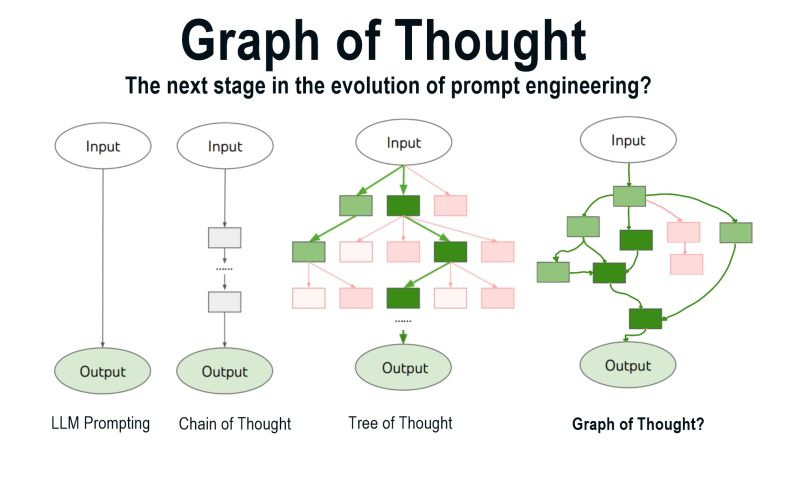
\includegraphics[width=\linewidth,keepaspectratio]{llm53}
\end{center}	

{\tiny (Ref: LinkedIn post by Tony Seale)}

	
\end{frame}



%%%%%%%%%%%%%%%%%%%%%%%%%%%%%%%%%%%%%%%%%%%%%%%%%%%%%%%%%%%
\begin{frame}[fragile]\frametitle{Conclusions}
\begin{itemize}
\item Graph-based Knowledge Graphs enhance LLMs in the enterprise context.
\item Leveraging Knowledge Graphs improves AI accuracy and relevance.
\item Benefits: Better data comprehension, refined compliance procedures, accelerated research and development.
\item CIOs should explore applying LLMs to internal data stores and constructing knowledge graphs using graph data science algorithms for substantial business breakthroughs.data science algorithms, as this strategy could yield substantial breakthroughs for their businesses.
\end{itemize}
\end{frame}


%%%%%%%%%%%%%%%%%%%%%%%%%%%%%%%%%%%%%%%%%%%%%%%%%%%%%%%%%%%
\begin{frame}[fragile]\frametitle{References}
\begin{itemize}
\item Knowledge Graphs \& LLMs: Fine-Tuning Vs. Retrieval-Augmented Generation - Tomaz Bratanic
\item Building knowledge graphs from unstructured data with OpenAI by Priyanka Shah
\item LLM’s Closing the KG Gap - Dean Allemang
\item The Future of Knowledge Graphs in a World of Large Language Models - Denny Vrandecic
\item Generating Company Recommendations using Large Language Models and Knowledge Graphs by Mike Tung
\item Large Language Model = Knowledge Graph Store? Yes, by Fine-Tuning LLM With KG - Peter Lawrence
\item Knowledge Graphs + Large Language Models = The ability for users to ask their own questions? - Peter Lawrence
\item Automatic Knowledge Graphs: The Impossible Grail - Patrick Meyer
\item Project NaLLM - https://github.com/neo4j/NaLLM
\item KELM: Integrating Knowledge Graphs with Language Model Pre-training Corpora 
\item How to use large language models and knowledge graphs to manage enterprise data 
\item Enhancing Large Language Models with Graph-based Knowledge Graphs: Overcoming Limitations and Unlocking Enterprise Potential - Nicholas Moss
\item ``Unifying Large Language Models and Knowledge Graphs: A Roadmap'' - Shirui Pan et al
\item LLM Ontology-prompting for Knowledge Graph Extraction - Peter Lawrence
\end{itemize}
\end{frame}

%%%%%%%%%%%%%%%%%%%%%%%%%%%%%%%%%%%%%%%%%%%%%%%%%%%%%%%%%%%
\begin{frame}[fragile]\frametitle{References}
\begin{itemize}
\item Exploring ChatGPT for Learning, Code, Data, NLP \& Fun
\item Create Neo4j Database Model with ChatGPT
\item ChatGPT and Neo4j for Creating and Importing Sample Datasets
\item Doctor.ai+GPT-3+Kendra = An Ensemble Chatbot for Healthcare
\item Creating a Knowledge Graph From Video Transcripts With ChatGPT
\item Context-Aware Knowledge Graph Chatbot With GPT-4 and Neo4j
\item Generating Company Recommendations using LLMs \& Knowledge Graphs
\item Integrating Neo4j into the LangChain ecosystem
\item Fine-tuning an LLM model with H2O LLM Studio to generate Cypher statements
\item Generating Cypher Queries With ChatGPT 4 on Any Graph Schema
\item ChatGPT Generated Star Wars Data: Let's Explore With Neo4j
\item LangChain has added Cypher Search
\item Knowledge Graphs \& LLMs: Harnessing Large Language Models with Neo4j
\item Jump into Graph: Creating Mock Data to get started with Graph Databases
\item Neo4j Live: GraphGPT
\item OpenAI API Access - APOC Extended Documentation
\item LangChain Cypher Search: Tips \& Tricks
\item Neo4j Integrations with Generative AI Features in Google Cloud Vertex AI
\item Neo4j Knowledge Graphs and Google Generative AI
\item Integrate LLM workflows with Knowledge Graph using Neo4j and APOC
\item Unifying Large Language Models and Knowledge Graphs: A Roadmap
\item Neo4j’s Role in Fueling Generative AI with Graph Technology
\item Knowledge Graphs \& LLMs: Fine-Tuning Vs. Retrieval-Augmented Generation
\item Knowledge Graphs \& LLMs: Multi-Hop Question Answering
\item Neo4j Knowledge Graphs and Google Generative AI
\item Personal Movie Recommendation Agent with GPT4 + Neo4j
\item Creating a Knowledge Graph From Video Transcripts With ChatGPT
\end{itemize}
\end{frame}